\section{Riemann Sums}\label{sec:riemann}

In the previous section we defined the definite integral of a function on $[a,b]$ to be the signed area between the curve and the $x$--axis. Some areas were simple to compute; we ended the section with a region whose area was not simple to compute. In this section we develop a technique to find such areas.\index{Riemann Sum}

A fundamental calculus technique is to first answer a given problem with an approximation, then refine that approximation to make it better, then use limits in the refining process to find the exact answer. That is  what we will do here.

Consider the region given in Figure \ref{fig:rie1a}, which is the area under $y=4x-x^2$ on $[0,4]$. What is the signed area of this region -- i.e., what is $\int_0^4(4x-x^2)\ dx$?

\mfigure{.75}{A graph of $f(x) = 4x-x^2$. What is the area of the shaded region?}{fig:rie1a}{figures/figrie1a}

We start by approximating. We can surround the region with a rectangle with height and width of 4 and find the area is approximately 16 square units. This is obviously an \textit{over--approximation}; we are including area in the rectangle that is not under the parabola. 

%We can try to compensate for this over--estimate by reducing the height of the rectangle. This would leave out some area, but still include too much in other places. We'd be guessing, though, as to the ``best'' height to choose.

We have an approximation of the area, using one rectangle. How can we refine our approximation to make it better? The key to this section is this answer: \textit{use more rectangles.}

Let's use 4 rectangles with an equal width of 1. This \textit{partitions} the interval $[0,4]$ into 4 \textit{subintervals}, $[0,1]$, $[1,2]$, $[2,3]$ and $[3,4]$. On each subinterval we will draw a rectangle.

There are three common ways to determine the height of these rectangles: the \textbf{Left Hand Rule}, the \textbf{Right Hand Rule}, and the \textbf{Midpoint Rule}. The \textbf{Left Hand Rule} says to evaluate the function at the left--hand endpoint of the subinterval and make the rectangle that height. In Figure \ref{fig:rie1b}, the rectangle drawn on the interval $[2,3]$ has height determined by the Left Hand Rule; it has a height of $f(2)$. (The rectangle is labeled ``LHR.'')\index{Left Hand Rule}\index{Right Hand Rule}\index{Midpoint Rule}

\mfigure{.5}{Approximating $\int_0^4(4x-x^2)\ dx$ using rectangles. The heights of the rectangles are determined using different rules.}{fig:rie1b}{figures/figrie1b}

The \textbf{Right Hand Rule} says the opposite: on each subinterval, evaluate the function at the right endpoint and make the rectangle that height. In the figure, the rectangle drawn on $[0,1]$ is drawn using $f(1)$ as its height; this rectangle is labeled ``RHR.''.

The \textbf{Midpoint Rule} says that on each subinterval, evaluate the function at the midpoint and make the rectangle that height. The rectangle drawn on $[1,2]$ was made using the Midpoint Rule, with a height of $f(1.5)$. That rectangle is labeled ``MPR.''

These are the three most common rules for determining the heights of approximating rectangles, but one is not forced to use one of these three methods. The rectangle on $[3,4]$ has a height of approximately $f(3.53)$, very close to the Midpoint Rule. It was chosen so that the area of the rectangle is \textit{exactly} the area of the region under $f$ on $[3,4]$. (Later you'll be able to figure how to do this, too.)

The following example will approximate the value of $\int_0^4 (4x-x^2)\ dx$ using these rules.\\

\example{ex_rie2}{Using the Left Hand, Right Hand and Midpoint Rules}{
Approximate the value of $\int_0^4 (4x-x^2)\ dx$ using the Left Hand Rule, the Right Hand Rule, and the Midpoint Rule, using 4 equally spaced subintervals.}
{We break the interval $[0,4]$ into four subintervals as before. In Figure \ref{fig:rie2}(a) we see 4 rectangles drawn on $f(x) = 4x-x^2$ using the Left Hand Rule. (The areas of the rectangles are given in each figure.)

%\mfigure{.8}{Approximating $\int_0^4(4x-x^2)\ dx$ using the Left Hand Rule in Example \ref{ex_rie2}.}{fig:rie2a}{figures/figrie2a}
%
\mtable{.6}{Approximating $\int_0^4(4x-x^2)\ dx$ in Example \ref{ex_rie2}. In (a), the Left Hand Rule is used; in (b), the Right Hand Rule is used; in (c), the Midpoint Rule is used.}{fig:rie2}{
\begin{tabular}{c}
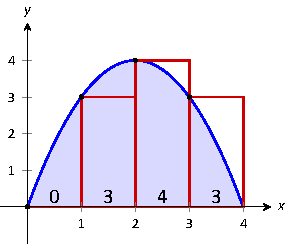
\includegraphics{figures/figrie2a}\\
(a)\\
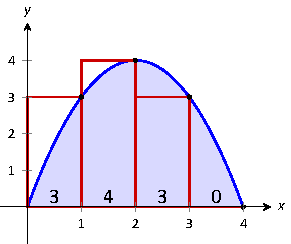
\includegraphics{figures/figrie2b}\\
(b)\\
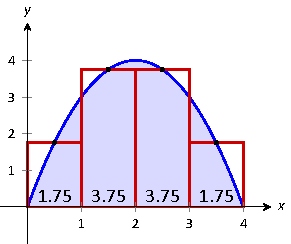
\includegraphics{figures/figrie2c}\\
(c)\\
\end{tabular}
}

%\noindent 
Note how in the first subinterval, $[0,1]$, the rectangle has height $f(0)=0$. We add up the areas of each rectangle (height$\times$ width) for our Left Hand Rule approximation:
	\begin{align*} f(0)\cdot 1 + f(1)\cdot 1+ f(2)\cdot 1+f(3)\cdot 1 &=\\
	0+3+4+3&= 10.
	\end{align*}
	
Figure \ref{fig:rie2}(b) shows 4 rectangles drawn under $f$ using the Right Hand Rule; note how the $[3,4]$ subinterval has a rectangle of height 0. 

%\mfigure{.57}{Approximating $\int_0^4(4x-x^2)\ dx$ using the Right Hand Rule in Example \ref{ex_rie2}.}{fig:rie2b}{figures/figrie2b}

%\noindent 
In this example, these rectangle seem to be the mirror image of those found in part (a) of the Figure. This is because of the symmetry of our shaded region. Our approximation gives the same answer as before, though calculated a different way:
	\begin{align*} f(1)\cdot 1 + f(2)\cdot 1+ f(3)\cdot 1+f(4)\cdot 1 &=\\
	3+4+3+0&= 10.
	\end{align*}

Figure \ref{fig:rie2}(c) shows 4 rectangles drawn under $f$ using the Midpoint Rule. 
%\mfigure{.35}{Approximating $\int_0^4(4x-x^2)\ dx$ using the Midpoint Rule in Example \ref{ex_rie2}.}{fig:rie2c}{figures/figrie2c}
This gives an approximation of $\int_0^4(4x-x^2)\ dx$ as:
\begin{align*} f(0.5)\cdot 1 + f(1.5)\cdot 1+ f(2.5)\cdot 1+f(3.5)\cdot 1 &=\\
	1.75+3.75+3.75+1.75&= 11.
	\end{align*}
Our three methods provide two approximations of $\int_0^4(4x-x^2)\ dx$: 10 and 11.
}\\

\noindent\textbf{\large Summation Notation}
\vskip\baselineskip
It is hard to tell at this moment which is a better approximation: 10 or 11? We can continue to refine our approximation by using more rectangles. The notation can become unwieldy, though, as we add up longer and longer lists of numbers. We introduce \textbf{summation notation} to ameliorate this problem. \index{summation!notation}

\clearpage

Suppose we wish to add up a list of numbers $a_1$, $a_2$, $a_3$, \ldots, $a_9$. Instead of writing $$a_1+a_2+a_3+a_4+a_5+a_6+a_7+a_8+a_9,$$ we use summation notation and write 
\begin{center}
\myincludegraphics{figures/figrie_notation}
\captionsetup{type=figure}%
\caption{Understanding summation notation.}\label{fig:rie_notation}
\end{center}

The upper case sigma represents the term ``sum.'' The index of summation in this example is $i$; any symbol can be used. By convention, the index takes on only the integer values between (and including) the lower and upper bounds. 

Let's practice using this notation.\\

\example{ex_rie3}{Using summation notation}{
Let the numbers $\{a_i\}$ be defined as $a_i = 2i-1$ for integers $i$, where $i\geq 1$. So $a_1 = 1$, $a_2 = 3$, $a_3 = 5$, etc. (The output is the positive odd integers). Evaluate the following summations:
$$ 1.\ \sum_{i=1}^6 a_i \qquad\qquad\qquad 2.\ \sum_{i=3}^7 (3a_i-4)\qquad\qquad \qquad 3.\ \sum_{i=1}^4 (a_i)^2$$
}
{\begin{enumerate}
		\item		\noindent\vskip-45pt%\begin{minipage}[t]{\linewidth}
						\begin{align*}
						\sum_{i=1}^6 a_i &= a_1+a_2+a_3+a_4+a_5+a_6\\
														&=	1+3+5+7+9+11 \\
														&=	36.
					\end{align*}
%					\end{minipage}
		\item	Note the starting value is different than 1:
					\begin{align*}
					\sum_{i=3}^7 (3a_i-4) &= (3a_3-4)+(3a_4-4)+(3a_5-4)+(3a_6-4)+(3a_7-4) \\
														&= 11+17+23+29+35 \\
														&= 115.
					\end{align*}
		\item		\noindent\vskip-45pt%\begin{minipage}[t]{\linewidth}
						\begin{align*}
						\sum_{i=1}^4 (a_i)^2 &=	(a_1)^2+(a_2)^2+(a_3)^2+(a_4)^2\\
																&=	1^2+3^2+5^2+7^2 \\
																&=	84.
						\end{align*}
\end{enumerate}	
\vskip-3\baselineskip											
}\\

It might seem odd to stress a new, concise way of writing summations only to write each term out as we add them up. It is. The following theorem gives some of the properties of summations that allow us to work with them without writing individual terms. Examples will follow.

\setboxwidth{75pt}
\theorem{thm:summation}{Properties of Summations}
{\noindent\begin{minipage}[t]{200pt}\index{summation!properties}
\begin{enumerate}
		\item		$\ds \sum_{i=1}^n c = c\cdot n$, where $c$ is a constant.
		\item		$\ds \sum_{i=m}^n (a_i\pm b_i) = \sum_{i=m}^n a_i \pm \sum_{i=m}^n b_i$
		\item		$\ds \sum_{i=m}^n c\cdot a_i = c\cdot\sum_{i=m}^n a_i$
		\item		$\ds \sum_{i=m}^j a_i + \sum_{i=j+1}^n  a_i = \sum_{i=m}^n a_i$
%		\item		$\ds \sum_{i=1}^n i = \frac{n(n+1)}2$
%		\item		$\ds \sum_{i=1}^n i^2 = \frac{n(n+1)(2n+1)}6$
%		\item		$\ds \sum_{i=1}^n i^3 = \left(\frac{n(n+1)}2\right)^2$
	\end{enumerate}
\end{minipage}
\begin{minipage}[t]{200pt}
\begin{enumerate}\addtocounter{enumi}{4}
%		\item		$\ds \sum_{i=1}^n c = c\cdot n$, where $c$ is a constant.
%		\item		$\ds \sum_{i=m}^n (a_i\pm b_i) = \sum_{i=m}^n a_i \pm \sum_{i=m}^n b_i$
%		\item		$\ds \sum_{i=1}^n c\cdot a_i = c\cdot\sum_{i=1}^n a_i$
%		\item		$\ds \sum_{i=m}^j a_i + \sum_{i=j+1}^n  a_i = \sum_{i=m}^n a_i$
		\item		$\ds \sum_{i=1}^n i = \frac{n(n+1)}2$
		\item		$\ds \sum_{i=1}^n i^2 = \frac{n(n+1)(2n+1)}6$
		\item		$\ds \sum_{i=1}^n i^3 = \left(\frac{n(n+1)}2\right)^2$
	\end{enumerate}
\end{minipage}
}
\restoreboxwidth

\example{ex_rie4}{Evaluating summations using Theorem \ref{thm:summation}}
{Revisit Example \ref{ex_rie3} and, using Theorem \ref{thm:summation}, evaluate $$\sum_{i=1}^6 a_i = \sum_{i=1}^6 (2i-1).$$
}
{\begin{align*}
		\sum_{i=1}^6 (2i-1) & = \sum_{i=1}^6 2i - \sum_{i=1}^6 (1)\\
												&=	\left(2\sum_{i=1}^6 i \right)- 6 \\
												&= 2\frac{6(6+1)}{2} - 6 \\
												&= 42-6 = 36
 \end{align*}
 We obtained the same answer without writing out all six terms. When dealing with small sizes of $n$, it may be faster to write the terms out by hand. However, Theorem \ref{thm:summation} is incredibly important when dealing with large sums as we'll soon see.
 }\\
 
\noindent\textbf{\large Riemann Sums}
\vskip \baselineskip

Consider again $\int_0^4(4x-x^2)\ dx$. We will approximate this definite integral using 16 equally spaced subintervals and the Right Hand Rule in Example \ref{ex_rie7}. Before doing so, it will pay  to do some careful preparation.\index{Riemann Sum}

\mfigure{.5}{Dividing $[0,4]$ into 16 equally spaced subintervals.}{fig:rie5}{figures/figrie5}

Figure \ref{fig:rie5} shows a number line of $[0,4]$ divided, or \textit{partitioned}, into 16 equally spaced subintervals. We denote $0$ as $x_1$; we have marked the values of $x_5$, $x_9$, $x_{13}$ and $x_{17}$. We could mark them all, but the figure would get crowded. While it is easy to figure that $x_{10} = 2.25$, in general, we want a method of determining the value of $x_i$ without consulting the figure. Consider:
	\begin{center}\myincludegraphics{figures/figrie5a}\end{center}
	%$$x_i = x_1 + (i-1)\Delta x. \text{TIKZ}$$
So $x_{10} = x_1 + 9(4/16) = 2.25.$

If we had partitioned $[0,4]$ into 100 equally spaced subintervals, each subinterval would have length $\Delta x=4/100 = 0.04$. We could compute $x_{32}$ as $$x_{32} = x_1 + 31(4/100) = 1.24.$$ (That was far faster than creating a sketch first.)

Given any subdivision of $[0,4]$, the first subinterval is $[x_1,x_2]$; the second is $[x_2,x_3]$; the $i^\text{ th}$ subinterval is $[x_i,x_{i+1}]$. 

When using the Left Hand Rule, the height of the $i^\text{ th}$ rectangle will be $f(x_i)$. 

When using the Right Hand Rule, the height of the $i^\text{ th}$ rectangle will be $f(x_{i+1})$. 

When using the Midpoint Rule, the height of the $i^\text{ th}$ rectangle will be $\ds f\left(\frac{x_i+x_{i+1}}2\right)$. 

Thus approximating $\int_0^4(4x-x^2)\ dx$ with 16 equally spaced subintervals can be expressed as follows, where $\Delta x = 4/16 = 1/4$:\vskip 5pt

\noindent \textbf{Left Hand Rule:} $\ds \sum_{i=1}^{16} f(x_i)\Delta x$ \vskip 5pt

\noindent \textbf{Right Hand Rule:} $\ds \sum_{i=1}^{16} f(x_{i+1})\Delta x$\vskip 5pt

\noindent \textbf{Midpoint Rule:} $\ds \sum_{i=1}^{16} f\left(\frac{x_i+x_{i+1}}2\right)\Delta x$
\index{Left Hand Rule}\index{Right Hand Rule}\index{Midpoint Rule}
\vskip 5pt

We use these formulas in the next two examples.
%\example{ex_rie6}{Use technology to approximate $\int_0^4(4x-x^2)\ dx$ using the Left Hand Rule and 16 and 100 equally spaced intervals. \\
%
%\mnote{.5}{\textbf{Note:} If one does not have ready access to such technology, one can still read and understand how technology can be used to accomplish these goals.}
%}
%{Consider first $n=16$. We have $\Delta x = 4/16 = 0.25$, and $x_i = (i-1)\Delta x$ (as worked out before). We want to evaluate $ \sum_{i=1}^{16} f(x_i)\Delta x$. Access to technology may vary; we show how to use \textit{Mathematica} to compute this sum.
%
%First, note that 
%\begin{align*}
%f(x_i) &= \parbox{130pt}{$\ds f\big(0+(i-1)\Delta x\big)$} \text{\small (using the formula for $x_i$)}\\
%			&= \parbox{130pt}{$\ds 4(i-1)\Delta x - \big((i-1)\Delta x\big)^2$} \text{\small (apply the formula $f(x) = 4x-x^2$)}\\
%			& = \parbox{130pt}{$\ds (i-1) - (.25(i-1))^2.$} \text{\small ($\Delta x = 0.25$)}
%\end{align*}
%
%We use the \texttt{Sum} command of \textit{Mathematica} to evaluate the summation using this latter expression of $f(x_i)$:
%\begin{center}
%\noindent\texttt{\detokenize{Sum[((i-1)-(0.25(i-1))^2)*(0.25),{i,1,16}]}}
%\end{center}
%\textit{Mathematica} takes virtually no time at all to return \texttt{10.625} as the sum, giving us a new (and likely better) approximation for $\int_0^4(4x-x^2)\ dx$.
%
%Once the groundwork is laid, it is easy to change from using 16 subintervals to 100. We now have $\Delta x=4/100 = 0.04$. Again simplify $f(x_i)$:
%\begin{align*}
%f(x_i) &= \parbox{130pt}{$\ds f\big(0+(i-1)\Delta x\big)$} \text{\small (using the formula for $x_i$)}\\
%			&= \parbox{130pt}{$\ds 4(i-1)\Delta x - \big((i-1)\Delta x\big)^2$} \text{\small (apply the formula $f(x) = 4x-x^2$)}\\
%			& = \parbox{130pt}{$\ds 0.16(i-1) - (.04(i-1))^2.$} \text{\small ($\Delta x = 0.04$)}
%\end{align*}
% We make the proper adjustments for $f(x_i)$ in our old \textit{Mathematica} expression, and  sum from $i=1$ to $i=100$:
%\begin{center}
%\noindent\texttt{\detokenize{Sum[(0.16(i-1)-(0.04(i-1))^2)*(0.04),{i,1,100}]}}
%\end{center}
%Again, \textit{Mathematica} nearly instantly computes this sum as \texttt{10.6656}.
%}\\
%
%One of the advantages of using a computer is that it can do a large number of calculations very quickly. Using 10,000 subintervals and the Left Hand Rule, \textit{Mathematica} took approximately $1/5^\text{ th}$ of a second to compute an approximation 10.66666656. It is worthwhile to ascertain what technology is available to you and to understand how to use it appropriately.
The following example lets us practice using the Right Hand Rule and the summation formulas introduced in Theorem \ref{thm:summation}.\\

\example{ex_rie7}{Approximating definite integrals using sums}{
Approximate $\int_0^4(4x-x^2)\ dx$ using the Right Hand Rule and summation formulas with 16 and 1000 equally spaced intervals.}
{Using the formula derived before, using 16 equally spaced intervals and the Right Hand Rule, we can approximate the definite integral as $$\sum_{i=1}^{16}f(x_{i+1})\Delta x.$$
We have $\Delta x = 4/16 = 0.25$. Since $x_i = 0+(i-1)\Delta x$, we have 
\begin{align*}
x_{i+1} &= 0 + \big((i+1)-1\big)\Delta x \\
				&=	i\Delta x
\end{align*}
%In our examples using the Right Hand Rule is simpler notationally as $f(x_{i+1}) = f(i\Delta x)$. 

Using the summation formulas, consider:
\begin{align}
\int_0^4 (4x-x^2)\ dx &\approx \sum_{i=1}^{16} f(x_{i+1})\Delta x \notag\\
											&= \sum_{i=1}^{16} f(i\Delta x) \Delta x\notag\\
									&= \sum_{i=1}^{16} \big(4i\Delta x - (i\Delta x)^2\big)\Delta x\notag\\
									&= \sum_{i=1}^{16} (4i\Delta x^2 - i^2\Delta x^3)\notag\\		
									&= (4\Delta x^2)\sum_{i=1}^{16} i - \Delta x^3 \sum_{i=1}^{16} i^2 \label{eq:rie7}\\
									&= (4\Delta x^2)\frac{16\cdot 17}{2} - \Delta x^3 \frac{16(17)(33)}6 \quad \text{\footnotesize $(\Delta x = 0.25)$}\notag\\
									%&=	4\cdot 0.25^2\cdot 136-0.25^3\cdot 1496\notag\\
									&=10.625\notag
\end{align}
We were able to sum up the areas of 16 rectangles with very little computation. In Figure \ref{fig:rie7} the function and the 16 rectangles are graphed. While some rectangles over--approximate the area, other under--approximate the area (by about the same amount). Thus our approximate area of 10.625 is likely a fairly good approximation.
\enlargethispage{3\baselineskip} 

Notice  Equation \eqref{eq:rie7}; by changing the 16's to 1,000's (and appropriately changing the value of $\Delta x$), we can use that equation to sum up 1000 rectangles!
%\drawexampleline
\mfigure{.5}{Approximating $\int_0^4(4x-x^2)\ dx$ with the Right Hand Rule and 16 evenly spaced subintervals.}{fig:rie7}{figures/figrie7}
%\enlargethispage{\baselineskip}
We do so here, skipping from the original summand to the equivalent of Equation \eqref{eq:rie7} to save space. Note that $\Delta x = 4/1000 = 0.004$.
\begin{align}
\int_0^4 (4x-x^2)\ dx &\approx \sum_{i=1}^{1000} f(x_{i+1})\Delta x \notag\\
									&= (4\Delta x^2)\sum_{i=1}^{1000} i - \Delta x^3 \sum_{i=1}^{1000} i^2 \notag\\
									&= (4\Delta x^2)\frac{1000\cdot 1001}{2} - \Delta x^3 \frac{1000(1001)(2001)}6 \notag\\
									%&=	4\cdot 0.004^2\cdot 500500-0.004^3\cdot 333,833,500\notag\\
									&=10.666656\notag
\end{align}

Using many, many rectangles, we have a likely good approximation of 

$\int_0^4 (4x-x^2)\dx$. That is, $$\int_0^4(4x-x^2)\ dx \approx 10.666656.$$
\vskip -1\baselineskip
}\\

Before the above example, we stated what the summations for the Left Hand, Right Hand and Midpoint Rules looked like. Each had the same basic structure, which was:
\begin{enumerate}
	\item each rectangle has the same width, which we referred to as $\Delta x$, and
	\item	each rectangle's height is determined by evaluating $f$ at a particular point in each subinterval. For instance, the Left Hand Rule states that each rectangle's height is determined by evaluating $f$ at the left hand endpoint of the subinterval the rectangle lives on.
\end{enumerate}
%; the only difference was at what values to evaluate $f$. 
One could partition an interval $[a,b]$ with subintervals that do not have the same size. We refer to the length of the %first subinterval as $\Delta x_1$, the length of the second subinterval as $\Delta x_2$, and so on, giving the length of the 
$i^\text{ th}$ subinterval as $\Delta x_i$. Also, one could determine each rectangle's height by evaluating $f$ at \emph{any} point $c_i$ in the $i^\text{ th}$ subinterval. %We refer to the point picked in the first subinterval as $c_1$, the point picked in the second subinterval as $c_2$, and so on, with $c_i$ representing the point picked in the $i^\text{ th}$ subinterval. 
Thus the height of the $i^\text{ th}$ subinterval would be $f(c_i)$, and the area of the $i^\text{ th}$ rectangle would be $f(c_i)\Delta x_i$. These ideas are formally defined below.
%\enlargethispage{4\baselineskip}

\definition{def:partition}{Partition}
{A \sword{partition} $\Delta x$ of a closed interval $[a,b]$ is a set of numbers $x_1$, $x_2$, $\ldots$ $x_{n+1}$ where 
$$a=x_1 < x_2 < \ldots < x_n < x_{n+1}=b.$$
The length of the $i^\text{ th}$ subinterval, $[x_i,x_{i+1}]$, is $\Delta x_i = x_{i+1}-x_i$. If $[a,b]$ is partitioned into subintervals of equal length, we let $\Delta x$ represent the length of each subinterval.\\

The \sword{size of the partition}, denoted $||\Delta x||$, is the length of the largest subinterval of the partition.\index{partition}\index{partition!size of}

%Let $f$ be defined on a closed interval $[a,b]$ and let $\Delta x$ be a partition of $[a,b]$, \index{Riemann Sum}
	%%$$a=x_1 < x_2 < \ldots < x_n < x_{n+1}=b.$$
%%Let $\Delta x_i$ denote the length of the $i^\text{ th}$ subinterval $[x_i,x_{i+1}]$ and 
%and let $c_i$ denote any value in the $i^\text{ th}$ subinterval.
%
%The sum $$\sum_{i=1}^n f(c_i)\Delta x_i$$  is a \textbf{Riemann sum} of $f$ on $[a,b]$.
}

Summations of rectangles with area $f(c_i)\Delta x_i$ are named after mathematician Georg Friedrich Bernhard Riemann, as given in the following definition.

%All three are examples of an even more general construction, named after mathematician Georg Friedrich Bernhard Riemann.

%In this general form, the subintervals do not have be of equal length, and one can choose a point $c_i$ inside each subinterval any way they choose (and not just the left endpoint, or the midpoint, etc.) Figure \ref{fig:riedef} shows the approximating rectangles of a Riemann sum of $\int_0^4(4x-x^2)\ dx$. (This particular approximation is of little use; clearly the width and heights of the rectangles were not chosen ``well.'')

\definition{def:rie_sum}{Riemann Sum}
{%
%A \sword{partition} $\Delta x$ of a closed interval $[a,b]$ is a set of numbers $x_1$, $x_2$, $\ldots$ $x_{n+1}$ where 
%$$a=x_1 < x_2 < \ldots < x_n < x_{n+1}=b.$$
%The length of the $i^\text{ th}$ subinterval is $\Delta x_i = x_{i+1}-x_i$. If $[a,b]$ is partitioned into subintervals of equal length, we let $\Delta x$ represent the length of each subinterval.\\
%
%The \sword{size of the partition}, denoted $||\Delta x||$, is the length of the largest subinterval of the partition.\index{partition}\index{partition!size of}\\
%
Let $f$ be defined on a closed interval $[a,b]$, let $\Delta x$ be a partition of $[a,b]$ \index{Riemann Sum}
	%$$a=x_1 < x_2 < \ldots < x_n < x_{n+1}=b.$$
%Let $\Delta x_i$ denote the length of the $i^\text{ th}$ subinterval $[x_i,x_{i+1}]$ and 
and let $c_i$ denote any value in the $i^\text{ th}$ subinterval.

The sum $$\sum_{i=1}^n f(c_i)\Delta x_i$$  is a \textbf{Riemann sum} of $f$ on $[a,b]$.}


Figure \ref{fig:riedef} shows the approximating rectangles of a Riemann sum of $\int_0^4(4x-x^2)\ dx$. While the rectangles in this example do not approximate well the shaded area, they demonstrate that the subinterval widths may vary and the heights of the rectangles can be determined without following a particular rule.
\mfigure{.8}{An example of a general Riemann sum to approximate $\int_0^4(4x-x^2)\ dx$.}{fig:riedef}{figures/figriedef}

``Usually'' Riemann sums are calculated using one of the three methods we have introduced. The uniformity of construction  makes computations easier. Before working another example, let's summarize some of what we have learned in a convenient way.
%\clearpage

%\enlargethispage{\baselineskip}
%\setboxwidth{50pt}
%\noindent\hskip-50pt\begin{minipage}{\specialboxlength}
\keyidea{idea:riemann}{Riemann Sum Concepts}
{Consider $\ds \int_a^b f(x) \ dx \approx \sum_{i=1}^n f(c_i)\Delta x_i.$ 

\begin{enumerate}
\item	When the $n$ subintervals have equal length, $\ds \Delta x_i = \Delta x = \frac{b-a}n.$
\item		The $i^\text{ th}$ term of an equally spaced partition is $x_i = a + (i-1)\Delta x$. (Thus $x_1=a$ and  $x_{n+1} = b$.)
\item		The Left Hand Rule summation is: $\ds \sum_{i=1}^n f(x_i)\Delta x$.
\item		The Right Hand Rule summation is: $\ds \sum_{i=1}^n f(x_{i+1})\Delta x$.
\item		The Midpoint Rule summation is: $\ds \sum_{i=1}^n f\left(\frac{x_i+x_{i+1}}{2}\right)\Delta x$.
\end{enumerate}
%\textit{\small (continued $\ldots$)}
}
%\end{minipage}
\restoreboxwidth
%\addtocounter{keyideacounter}{-1}
%
%\setboxwidth{60pt}
%\noindent\hskip-60pt
%\begin{minipage}{\specialboxlength}
%\keyidea{idea:riemannb}{Riemann Sum Concepts -- Continued}
%{Consider $\ds \int_a^b f(x) \ dx \approx \sum_{i=1}^n f(c_i)\Delta x_i.$ 
%
%\begin{enumerate}\addtocounter{enumi}{2}
%%\item	When the $n$ subintervals have equal length, $\ds \Delta x_i = \Delta x = \frac{b-a}n.$
%%\item		The $i^\text{ th}$ term of the partition is $x_i = a + (i-1)\Delta x$. (This makes $x_{n+1} = b$.)
%\item		\parbox{240pt}{The Left Hand Rule summation is: $\ds \sum_{i=1}^n f(x_i)\Delta x$}$(c_i=x_i)$.
%\item		\parbox{240pt}{The Right Hand Rule summation is: $\ds \sum_{i=1}^n f(x_{i+1})\Delta x$}$(c_i=x_{i+1})$.
%\item		\parbox{240pt}{The Midpoint Rule summation is: $\ds \sum_{i=1}^n f\left(\frac{x_i+x_{i+1}}{2}\right)\Delta x$}$(c_i=(x_i+x_{i+1})/2)$.\index{Left Hand Rule}\index{Right Hand Rule}\index{Midpoint Rule}
%
%\end{enumerate}
%}
%\end{minipage}
%\restoreboxwidth


Let's do another example.\\

\example{ex_rie8}{Approximating definite integrals with sums}{
Approximate $\int_{-2}^3 (5x+2)\ dx$ using the Midpoint Rule and 10 equally spaced intervals.}
{Following Key Idea \ref{idea:riemann}, we have
	$$\Delta x = \frac{3 - (-2)}{10} = 1/2 \quad \text{and} \quad x_i = (-2) + (1/2)(i-1) = i/2-5/2.$$
	As we are using the Midpoint Rule, we will also need $x_{i+1}$ and $\ds \frac{x_i+x_{i+1}}2$. Since $x_i = i/2-5/2$,\quad $x_{i+1} = (i+1)/2 - 5/2 = i/2 -2$.
	This gives 
	$$\frac{x_i+x_{i+1}}2 = \frac{(i/2-5/2) + (i/2-2)}{2} = \frac{i-9/2}{2} = i/2 - 9/4.$$
	We now construct the Riemann sum and compute its value using summation formulas.
\begin{align*}
\int_{-2}^3 (5x+2)\ dx 	&\approx \sum_{i=1}^{10} f\left(\frac{x_i+x_{i+1}}{2}\right)\Delta x \\
												&=	\sum_{i=1}^{10} f(i/2 - 9/4)\Delta x \\
												&=	\sum_{i=1}^{10} \big(5(i/2-9/4) + 2\big)\Delta x\\
												&=	\Delta x\sum_{i=1}^{10}\left[\left(\frac{5}{2}\right)i - \frac{37}{4}\right]\\
												&=	\Delta x\left(\frac{5}2\sum_{i=1}^{10} (i) - \sum_{i=1}^{10}\left(\frac{37}{4}\right)\right) \\
												&= \frac12\left(\frac52\cdot\frac{10(11)}{2} - 10\cdot\frac{37}4\right)  \\
												&= \frac{45}2 = 22.5
\end{align*}
\mfigure{.55}{Approximating $\int_{-2}^3 (5x+2)\ dx$ using the Midpoint Rule and 10 evenly spaced subintervals in Example \ref{ex_rie8}.}{fig:rie8}{figures/figrie8}

Note the graph of $f(x) = 5x+2$ in Figure \ref{fig:rie8}. The regions whose area is computed by the definite integral are triangles, meaning we can find the exact answer without summation techniques. We find that the exact answer is indeed 22.5. One of the strengths of the Midpoint Rule is that often each rectangle includes area that should not be counted, but misses other area that should. When the partition size is small, these two amounts are about equal and these errors almost ``cancel each other out.'' In this example, since our function is a line, these errors are exactly equal and they do cancel each other out, giving us the exact answer.

Note too that when the function is negative, the rectangles have a ``negative'' height. When we compute the area of the rectangle, we use $f(c_i)\Delta x$; when $f$ is negative, the area is counted as negative.
}\\

Notice in the previous example that while we used 10 equally spaced intervals, the number ``10'' didn't play a big role in the calculations until the very end. Mathematicians love to abstract ideas; let's approximate the area of another region using $n$ subintervals, where we do not specify a value of $n$ until the very end.\\

\example{ex_rie9}{Approximating definite integrals with a formula, using sums}{
Revisit $\int_0^4(4x-x^2)\ dx$ yet again. Approximate this definite integral using the Right Hand Rule with $n$ equally spaced subintervals.}
{Using Key Idea \ref{idea:riemann}, we know $\Delta x = \frac{4-0}{n} = 4/n$. We also find $x_i = 0 + \Delta x(i-1) = 4(i-1)/n$. The Right Hand Rule uses $x_{i+1}$, which is $x_{i+1} = 4i/n$.

We construct the Right Hand Rule Riemann sum as follows. Be sure to follow each step carefully. If you get stuck, and do not understand how one line proceeds to the next, you may skip to the result and consider how this result is used. You should come back, though, and work through each step for full understanding.
\begin{align*}
		\int_0^4(4x-x^2)\ dx &\approx \sum_{i=1}^n f(x_{i+1})\Delta x \\
											&= \sum_{i=1}^n f\left(\frac{4i}{n}\right) \Delta x \\
											&=	\sum_{i=1}^n \left[4\frac{4i}n-\left(\frac{4i}n\right)^2\right]\Delta x\\
											&=	\sum_{i=1}^n \left(\frac{16\Delta x}{n}\right)i - \sum_{i=1}^n \left(\frac{16\Delta x}{n^2}\right)i^2 \\
											&=	\left(\frac{16\Delta x}{n}\right)\sum_{i=1}^n i - \left(\frac{16\Delta x}{n^2}\right)\sum_{i=1}^n i^2  \\
											&= \left(\frac{16\Delta x}{n}\right)\cdot \frac{n(n+1)}{2} - \left(\frac{16\Delta x}{n^2}\right)\frac{n(n+1)(2n+1)}{6} \quad \left(\parbox{35pt}{\scriptsize \centering recall $\Delta x = 4/n$}\right)\\
											&=\frac{32(n+1)}{n} - \frac{32(n+1)(2n+1)}{3n^2} \quad \text{\scriptsize (now simplify)} \\
											&= \frac{32}{3}\left(1-\frac{1}{n^2}\right)
\end{align*}
%\drawexampleline

The result is an amazing, easy to use formula. To approximate the definite integral with 10 equally spaced subintervals and the Right Hand Rule, set $n=10$ and compute $$\int_0^4 (4x-x^2)\ dx \approx \frac{32}{3}\left(1-\frac{1}{10^2}\right) = 10.56.$$
Recall how earlier we approximated the definite integral with 4 subintervals; with $n=4$, the formula gives 10, our answer as before.

It is now easy to approximate the integral with 1,000,000 subintervals!  Hand-held calculators will round off the answer a bit prematurely giving an answer of $10.66666667$. (The actual answer is $10.666666666656$.)

We now take an important leap. Up to this point, our mathematics has been limited to geometry and algebra (finding areas and manipulating expressions). Now we apply \textit{calculus}. For any \textit{finite} $n$, we know that $$\int_0^4 (4x-x^2)\ dx \approx \frac{32}{3}\left(1-\frac{1}{n^2}\right).$$ Both common sense and high--level mathematics tell us that as $n$ gets large, the approximation gets better. In fact, if we take the \textit{limit} as $n\rightarrow \infty$, we get the \textit{exact area} described by $\int_0^4 (4x-x^2)\ dx$. That is, 
\begin{align*}
\int_0^4 (4x-x^2)\ dx &= \lim_{n\rightarrow \infty} \frac{32}{3}\left(1-\frac{1}{n^2}\right) \\
									&= \frac{32}{3}\left(1-0\right)\\
									&= \frac{32}{3} = 10.\overline{6}
\end{align*}
This is a fantastic result. By considering $n$ equally--spaced subintervals, we obtained a formula for an approximation of the definite integral that involved our variable $n$. As $n$ grows large -- without bound -- the error shrinks to zero and we obtain the exact area.
}\\

This section started with a fundamental calculus technique: make an approximation, refine the approximation to make it better, then use limits in the refining process to get an exact answer. That is precisely what we just did.

Let's practice this again.\\

\example{ex_rie10}{Approximating definite integrals with a formula, using sums}{
Find a formula that approximates $\int_{-1}^5 x^3\ dx$ using the Right Hand Rule and $n$ equally spaced subintervals, then take the limit as $n\to\infty$ to find the exact area.}
{Following Key Idea \ref{idea:riemann}, we have $\Delta x = \frac{5-(-1)}{n} = 6/n$. We have $x_i = (-1) + (i-1)\Delta x$; as the Right Hand Rule uses $x_{i+1}$, we have $x_{i+1} = (-1) + i\Delta x$.

The Riemann sum corresponding to the Right Hand Rule is (followed by simplifications):
\begin{align*}
\int_{-1}^5 x^3\ dx 	&\approx \sum_{i=1}^n f(x_{i+1})\Delta x \\
											&= \sum_{i=1}^n f(-1+i\Delta x)\Delta x \\
											&= \sum_{i=1}^n (-1+i\Delta x)^3\Delta x \\
											&= \sum_{i=1}^n \big((i\Delta x)^3 -3(i\Delta x)^2 + 3i\Delta x -1\big)\Delta x \quad \text{\scriptsize (now distribute $\Delta x$)} \\
											&= \sum_{i=1}^n \big(i^3\Delta x^4 - 3i^2\Delta x^3 + 3i\Delta x^2 -\Delta x\big) \quad \text{\scriptsize (now split up summation)}\\
%\end{align*}
%\begin{align*}
											&= \Delta x^4 \sum_{i=1}^ni^3 -3\Delta x^3 \sum_{i=1}^n i^2+ 3\Delta x^2 \sum_{i=1}^n i - \sum_{i=1}^n \Delta x \\
											&= \Delta x^4 \left(\frac{n(n+1)}{2}\right)^2 -3\Delta x^3 \frac{n(n+1)(2n+1)}{6}+ 3\Delta x^2 \frac{n(n+1)}{2} - n\Delta x \\
											\intertext{\scriptsize (use $\Delta x = 6/n$)}
											&= \frac{1296}{n^4}\cdot\frac{n^2(n+1)^2}{4} - 3\frac{216}{n^3}\cdot\frac{n(n+1)(2n+1)}{6} + 3\frac{36}{n^2}\frac{n(n+1)}2 -6
											\intertext{\scriptsize (now do a sizable amount of algebra to simplify)}
											&=156 + \frac{378}n + \frac{216}{n^2}
\end{align*}
Once again, we have found a compact formula for approximating the definite integral with $n$ equally spaced subintervals and the Right Hand Rule. Using 10 subintervals, we have an approximation of $195.96$ (these rectangles are shown in Figure \ref{fig:rie9}). Using $n=100$ gives an approximation of $159.802$. 

\mfigure{.5}{Approximating $\int_{-1}^5 x^3\ dx$ using the Right Hand Rule and 10 evenly spaced subintervals.}{fig:rie9}{figures/figrie9}

Now find the exact answer using a limit:
$$\int_{-1}^5 x^3\ dx = \lim_{n\to\infty} \left(156 + \frac{378}n + \frac{216}{n^2}\right) = 156.$$
\vskip-\baselineskip
}\\

\noindent\textbf{\large Limits of Riemann Sums}
\vskip \baselineskip

We have used limits to evaluate given definite integrals. Will this always work? We will show, given not--very--restrictive conditions, that yes, it will always work.

The previous two examples demonstrated how an expression such as $$\sum_{i=1}^n f(x_{i+1})\Delta x$$ can be rewritten as an expression explicitly involving $n$, such as $32/3(1-1/n^2)$. 

Viewed in this manner, we can think of the summation as a function of $n$. An $n$ value is given (where $n$ is a positive integer), and the sum of areas of $n$ equally spaced rectangles is returned, using the Left Hand, Right Hand, or Midpoint Rules. 

Given a definite integral $\int_a^b f(x)\ dx$, let:
	\begin{itemize}
	\item	$\ds S_L(n) = \sum_{i=1}^n f(x_i)\Delta x$, the sum of equally spaced rectangles formed using the Left Hand Rule,
	\item	$\ds S_R(n) = \sum_{i=1}^n f(x_{i+1})\Delta x$, the sum of equally spaced rectangles formed using the Right Hand Rule, and
	\item	$\ds S_M(n) = \sum_{i=1}^n f\left(\frac{x_i+x_{i+1}}{2}\right)\Delta x$, the sum of equally spaced rectangles formed using the Midpoint Rule.
	\end{itemize}
	
Recall the definition of a limit as $n\to\infty$: 
		$\ds\lim_{n\to\infty}S_L(n) = K$ if, given any $\epsilon>0$, there exists $N>0$ such that 
		$$\left|S_L(n)-K\right| < \epsilon \quad \text{when}\quad n\geq N.$$

The following theorem states that we can use any of our three rules to find the exact value of a definite integral $\int_a^b f(x)\ dx$. It also goes two steps further. The theorem states that the height of each rectangle doesn't have to be determined following a specific rule, but could be $f(c_i)$, where $c_i$ is any point in the $i^\text{ th}$ subinterval, as discussed before Riemann Sums where defined in Definition \ref{def:rie_sum}.

The theorem goes on to state that the rectangles do not need to be of the same width. Using the notation of Definition \ref{def:partition}, let $\Delta x_i$ denote the length of the $i^\text{ th}$ subinterval in a partition of $[a,b]$ and let $||\Delta x||$ represent the length of the largest subinterval in the partition: that is, $||\Delta x||$ is the largest of all the $\Delta x_i$'s. If $||\Delta x||$ is small, then $[a,b]$ must be partitioned into many subintervals, since all subintervals must have small lengths. ``Taking the limit as $||\Delta x||$ goes to zero'' implies that the number $n$ of subintervals in the partition is growing to infinity, as the largest subinterval length is becoming arbitrarily small. We then interpret the expression 
$$\lim_{||\Delta x||\to 0}\sum_{i=1}^nf(c_i)\Delta x_i$$
as ``the limit of the sum of the areas of rectangles, where the width of each rectangle can be different but getting small, and the height of each rectangle is not necessarily determined by a particular rule.'' The theorem states that this Riemann Sum also gives the value of the definite integral of $f$ over $[a,b]$.

%Let $\Delta x$ represent \textit{any} partition of $[a,b]$, and let $\|\Delta x\|$ denote the length of the longest subinterval of this partition. The theorem also states that limit of \textit{any} Riemann sum of the form $\sum_{i=1}^n f(c_i)\Delta x_i$, as $\|\Delta x\|\to 0$, also gives the exact value of the definite integral.

%\setboxwidth{5pt}
%\noindent\hskip-5pt
%\begin{minipage}{\specialboxlength}
\theorem{thm:riemann_sum}{Definite Integrals and the Limit of Riemann Sums}
{Let $f$ be continuous on the closed interval $[a,b]$  and let $S_L(n)$, $S_R(n)$, $S_M(n)$, $\Delta x$, $\Delta x_i$ and $c_i$ be defined as before. Then:\index{Riemann Sum!and definite integral}\index{integration!definite!Riemann Sums}
\begin{enumerate}
	\item		$\ds \lim_{n\to\infty} S_L(n) = \lim_{n\to\infty} S_R(n) = \lim_{n\to\infty} S_M(n) = \lim_{n\to\infty}\sum_{i=1}^n f(c_i)\Delta x$, 
	
	\item		$\ds \lim_{n\to\infty}\sum_{i=1}^n f(c_i)\Delta x = \int_a^b f(x)\ dx$, and %$\ds \lim_{n\to\infty} S_L(n) = \int_a^b f(x)\ dx$.
	\item		$\ds \lim_{\|\Delta x\|\to 0} \sum_{i=1}^n f(c_i)\Delta x_i = \int_a^b f(x)\ dx$.%, where the latter sum is any Riemann sum of $f$ on $[a,b]$, and
\end{enumerate}
}
%\end{minipage}
%\restoreboxwidth

We summarize what we have learned over the past few sections here.
\begin{itemize}
\item		Knowing the ``area under the curve'' can be useful. One common example: the area under a velocity curve is displacement.
\item		We have defined the definite integral, $\int_a^b f(x)\ dx$, to be the signed area under $f$ on the interval $[a,b]$. 
\item		While we can approximate a definite integral many ways, we have focused on using rectangles whose heights can be determined using the Left Hand Rule, the Right Hand Rule and the Midpoint Rule. 
\item		Sums of rectangles of this type are called Riemann sums.
\item		The exact value of the definite integral can be computed using the limit of a Riemann sum. We generally use one of the above methods as it makes the algebra simpler.
\end{itemize}

We first learned of derivatives through limits then learned rules that made the process simpler. We know of a way to evaluate a definite integral using limits; in the next section we will see how the Fundamental Theorem of Calculus makes the process simpler. The key feature of this theorem is its connection between the indefinite integral and the definite integral.

\printexercises{exercises/05_03_exercises}